%\renewcommand{\lastmod}{April 29, 2020}

\chapter{Kristallgitter}





\section{Ziele}

\begin{itemize}

\item Sie können das Konzept von mathematischem Punktgitter und physikalischer Basis benutzen, um Strukturen wie die unten gezeigte zu beschreiben.

\item Sie können die konventionelle Einheitszelle der häufigsten Bravais-Gitter erkennen und zeichnen, sowie die Wigner-Seitz-Zelle konstruieren.

\item Sie können die verschiedenen Arten der Bindung in einem Festkörper erklären und dabei das Konzept der Madelung-Konstante verwenden.

\end{itemize}


\begin{figure}
\inputtikz{\currfiledir intro}
%  \caption{Absorptions- und Fluoreszenz-Spektrum des Farbstoffs BODIPY  (\href{https://www.thermofisher.com/de/de/home/life-science/cell-analysis/labeling-chemistry/fluorescence-spectraviewer.html?SID=srch-svtool&UID=10001moh}{thermofischer.com}).}
\end{figure}



\section{Überblick}

Die Festkörperphysik demonstriert Lösungen für das Problem, ein System aus sehr viele Teilchen einfach zu beschreiben. In der Atomphysik haben wir einen Kern und im Wesentlichen ein Elektron betrachtet. Weitere Elektronen sind hinzugekommen, deren Wechselwirkung wurde aber quasi vernachlässigt. In der Molekülphysik hatten wir mehrere Atome, oft zwei, manchmal etwa 10. Wieder haben wir das System oft auf die Bewegung einer reduzierten Masse vereinfacht. Im Hückel-verfahren hatten wir eine Methode gesehen, mit der man viele Atome in einem Molekül behandeln kann. In der Festkörperphysik müssen aber nicht ein paar 10 oder 100 Atome, sondern etwa $10^{23}$ Atome behandelt werden. Das Diagonalisieren einer Matrix dieser Kantenlänge ist sicherlich unpraktikabel.

Die Festkörperphysik führt zu diesem Zweck Konzepte zur Behandlung sehr großer Systeme ein. Aus meiner Sicht sind die wesentlichen Konzepte 
\begin{itemize} \setlength{\itemsep}{0pt}
\item das {Kristallgitter}
\item der {reziproke Raum} als Fourier-Transformierte des Kristallgitters
\item das Quasi-Teilchen als Anregung eines Vielteilchen-Systems, die sich wie ein Teilchen benimmt
\item die Dispersionsrelation als Energie-Impuls-Darstellung, die zur Bandstruktur führt
\end{itemize}
In den folgenden vier Kapiteln werden wir diese Konzepte anhand der Kerne in einem Festkörper einführen und deren Effekte diskutieren. Im nächsten Semester in der Festkörperphysik II werden dann Effekte der Elektronen in Festkörpern besprochen werden. Dies ist dann auch das 'modernste' Kapitel der kanonischen Experimentalphysik mit Effekten wie der Supraleitung und dem Quanten-Hall-Effekt.

Wir betrachten hier und im Wesentlichen auch im nächsten Semester nur kristalline, also periodische Festkörper. Man kann die Festkörperphysik als Untermenge der Physik der kondensierten Materie betrachten, in der dann auch amorphe, also nicht-kristalline Festkörper sowie Flüssigkeiten, Gläser und Polymere betrachtet werden. Dies ist dann Thema von Spezialveranstaltungen im Master-Studiengang. 

In diesem Kapitel werden wir die Idee eines Kristallgitters einführen und Methoden zu seiner Beschreibung besprechen. Das sind sozusagen die 'Vokabeln', die wir für die folgenden Kapitel benötigen.


\section{Bravais-Gitter}

Eine Kristallstruktur besteht aus einem mathematischen Punktgitter und einer Basis,  die die Physik in Form von einem oder mehreren Atomen beinhaltet. Man kann sich die Basis als Kachel vorstellen, die entsprechend dem Muster des Punktgitters angeordnet wird. Wie wir sehen werden ist dabei die Wahl der Basis nicht eindeutig. Zunächst betrachten wir nur das mathematische Punktgitter. Dies trägt den Namen von Auguste Bravais.

Ein dreidimensionales (mathematische) Gitter ist eine Anordnung von (mathematischen) Punkten im Raum, die translationsinvariant ist unter jeder Translation $\mathbf{T}$
\begin{equation}
 \mathbf{T} = n_1 \mathbf{a}_1 + n_2 \mathbf{a}_2 + n_3 \mathbf{a}_3  
\end{equation}
wobei die $n_i$ beliebige ganze Zahlen sind und die \emph{Basis-Vektoren} $\mathbf{a}_i$ nicht alle in einer Ebene liegen. Das 'Basis' in diesen Basis-Vektoren hat nichts mit der oben genannten Basis zu tun, die die Physik beinhaltet. Ein beliebiger Vektor aus der Menge der möglichen Translationen $\mathbf{T}$ wird als \emph{Gittervektor} bezeichnet. Die Länge der Basis-Vektoren   $\mathbf{a}_i$, also  $a_i$, wird \emph{Gitterkonstante} genannt.

\begin{marginfigure}
\inputtikz{\currfiledir einheitszelle}

\caption{Primitive (dunkelgrau) und nicht-primitive (hellgrau) Basis-Vektoren und Einheitszellen.}
\end{marginfigure}


Die Wahl der Basis-Vektoren   $\mathbf{a}_i$ ist  bei gegebenem Punktgitter nicht eindeutig. Zum einen sind Linearkombinationen von  Basis-Vektoren ebenfalls möglich, zum anderen verlangt unsere Definition von $\mathbf{T}$ nicht, dass \emph{jeder} Gitterpunkt durch die Translation $\mathbf{T}$  erreicht werden muss.  $\mathbf{a}'_i = 2 \mathbf{a}_i$ ist also ebenfalls möglich. Wir grenzen die Wahl etwas ein, indem wir das durch die Basis-Vektoren   $\mathbf{a}_i$  definierte Volumen betrachten. Dies ist die \emph{Elementarzelle} oder \emph{Einheitszelle}. Basis-Vektoren, die das kleinste Volumen aufspannen, nennt man \emph{primitiven Basis-Vektoren} bzw. deren Volumen die \emph{primitive Einheitszelle}. Diese Einheitszelle beinhaltet nur einen Gitterpunkt.\sidenote{Wenn man Punkte an Seiten, Ecken, Kanten der Einheitszelle anteilig rechnet.} Allerdings sind auch die primitiven Basis-Vektoren immer noch nicht eindeutig. Wir werden weiter unten in der Wigner-Seitz-Zelle eine eindeutig definierte primitive Einheitszelle kennenlernen.

Wenn also die $\mathbf{a}_i$ primitive  Basis-Vektoren sind, dann sind \emph{alle} Punkte des Gitters durch 
\begin{equation}
 \mathbf{R} = n_1 \mathbf{a}_1 + n_2 \mathbf{a}_2 + n_3 \mathbf{a}_3  
\end{equation}
mit ganzzahligen  $n_i$ beschrieben. Eine äquivalente Definition des Bravais-Gitters ist, dass Anordnung und Orientierung der Gitterpunkte von jedem Gitterpunkt aus gesehen gleich aussieht.


\section{Klassifizieren von Bravais-Gittern durch deren Symmetrie}

Wieviel verschiedene Punktgitter kann es im dreidimensionalen Raum geben? Ein Gitter gilt dann als 'verschieden', wenn es eine andere Symmetrie besitzt. Einfach alle Achsen skalieren ändert nichts Relevantes. Mögliche Symmetrie-Operationen sind die oben eingeführten Translationen $\mathbf{T}$. Eine andere Art von Symmetrie-Operationen lässt einen einzelnen Gitterpunkt unverändert. Die Menge dieser Operationen nennt man \emph{Punktgruppe} und ist Teil der Gruppentheorie.

\paragraph{Drehung} Was ist der kleinste Winkel $\phi$, um den man ein Gitter drehen kann, so dass es wieder in sich über geht? Dieser Winkel wird in der Form $\phi = 2 \pi / n$ als Zähligkeit $n$ notiert\sidenote{Dies ist die Notation nach Hermann-Mauguin. Alternativ gibt es auch die nach Schoenflies, hier $C_1$, $C_2$ etc.}. Es können nur Werte $n= 1$, 2, 3, 4 und 6 auftreten. Auch im Zweidimensionalen gibt es keine Kacheln mit 5, 7 oder 8 Ecken.

\paragraph{Spiegelung} Bei der Spiegelung an einer Ebene wird nicht nur ein Punkt sondern eine ganze Ebene, in der er liegt, festgehalten. Diese Symmetrie wird durch ein $m$ gekennzeichnet, wenn die Drehachse in dieser Spiegel-Ebene liegt, und durch $/m$, wenn die Drehachse senkrecht auf der Spiegel-Ebene steht.

\paragraph{Inversion} Die Punktspiegelung wird durch $\bar{1}$ gekennzeichnet.

\paragraph{Drehinversion} Dies ist eine hilfreiche zusammengesetzte Symmetrie-Operation aus einer Drehung und anschließender Inversion, die durch die Zähligkeit mit Überstrich, also beispielsweise $\bar{3}$ dargestellt wird. 

Auf Basis der Dreh-Symmetrie\footcite{Hunklinger2014} können die mathematischen Punkt-Gitter in sieben Klassen unterteilt werden, die sogenannten Kristallsysteme. Im kubischen System gibt es also 4 Rotationsachsen mit jeweils dreizähliger Symmetrie, die vier Raumdiagonalen des Würfels. Die anderen Symmetrie-Operationen werden eine Rolle spielen, wenn wir eine Basis an das mathematische Gitter binden.



\begin{table}
\begin{tabular}{llll}
Kristallsystem 	& 	Symmetrie & Gitterkonstante & Winkel \\
triklin 	&  	$1$						& $a_1 \neq a_2 \neq a_3$ &  $\alpha \neq \beta \neq \gamma$\\
monoklin 	& 	 $2$ 					& $a_1 \neq a_2 \neq a_3$ &  $\alpha = \gamma = 90^\circ, \beta \neq 90^\circ$\\
orthorhombisch 	& 	  $22$  & $a_1 \neq a_2 \neq a_3$ &  $\alpha= \beta =  \gamma = 90^\circ$\\
%
tetragonal 	&  $4$ & $a_1 = a_2 \neq a_3$ &   $\alpha= \beta =  \gamma = 90^\circ$\\
 hexagonal 	& 	 $6$ & $a_1 = a_2 \neq a_3$ &  $\alpha = \beta = 90^\circ, \gamma = 120^\circ$\\
trigonal 	& 	  $3$  & $a_1 = a_2 = a_3$ &  $\alpha = \beta = \gamma \neq 90^\circ$\\
kubisch 	&  	$3333$  & $a_1= a_2=  a_3$ &  $\alpha= \beta =  \gamma = 90^\circ$\\
\end{tabular}
\caption{Die sieben Kristallsysteme. 
 Der Winkel $\alpha$ wird von $\mathbf{a}_2$ und  $\mathbf{a}_3$  eingeschlossen, etc.}
\end{table}


Man kann die sieben Kristallsysteme weiter unterteilen\footcite{Bergmann-Schaefer-FK,AshcroftMermin2013} durch Hinzunehmen der Translationssymmetrie $\mathbf{T}$. Effektiv bedeutet dies, dass wo möglich weitere Gitterpunkte hinzugefügt werden, wobei aber die  Rotationssymmtrie der Kristallsysteme erhalten bleibt. 
Dies führt auf die 14 Bravais-Gitter, die in Abbildung \ref{fig:gitter_bravais14} gezeigt sind. Es ist die Leistung von Auguste Bravais zu erkennen, dass es genau diese und keine weiteren mathematisch Punktgitter gibt. Gitter ohne zusätzliche Punkte werden primitiv genannt, die mit hinzugefügten Punkten basis-, flächen- oder raum-zentriert. Diese Punkte sind natürlich ebenfalls Gitterpunkte, völlig äquivalent zu den an den Ecken gezeichneten Punkten. Alle Punkte sind gleich. Man könnte für die Zeichnung einen anderen Satz Punkte aus der unendlichen Menge der Gitterpunkte herausgreifen, und dann könnten diese Punkte an den Ecken der Darstellung liegen. Damit sind die gezeigten Strukturen, die \emph{konventionellen Einheitszellen}, nur im Fall der primitiven Gitter auch primitive Einheitszellen, ansonsten gewöhnliche  Einheitszellen.



\begin{figure}
%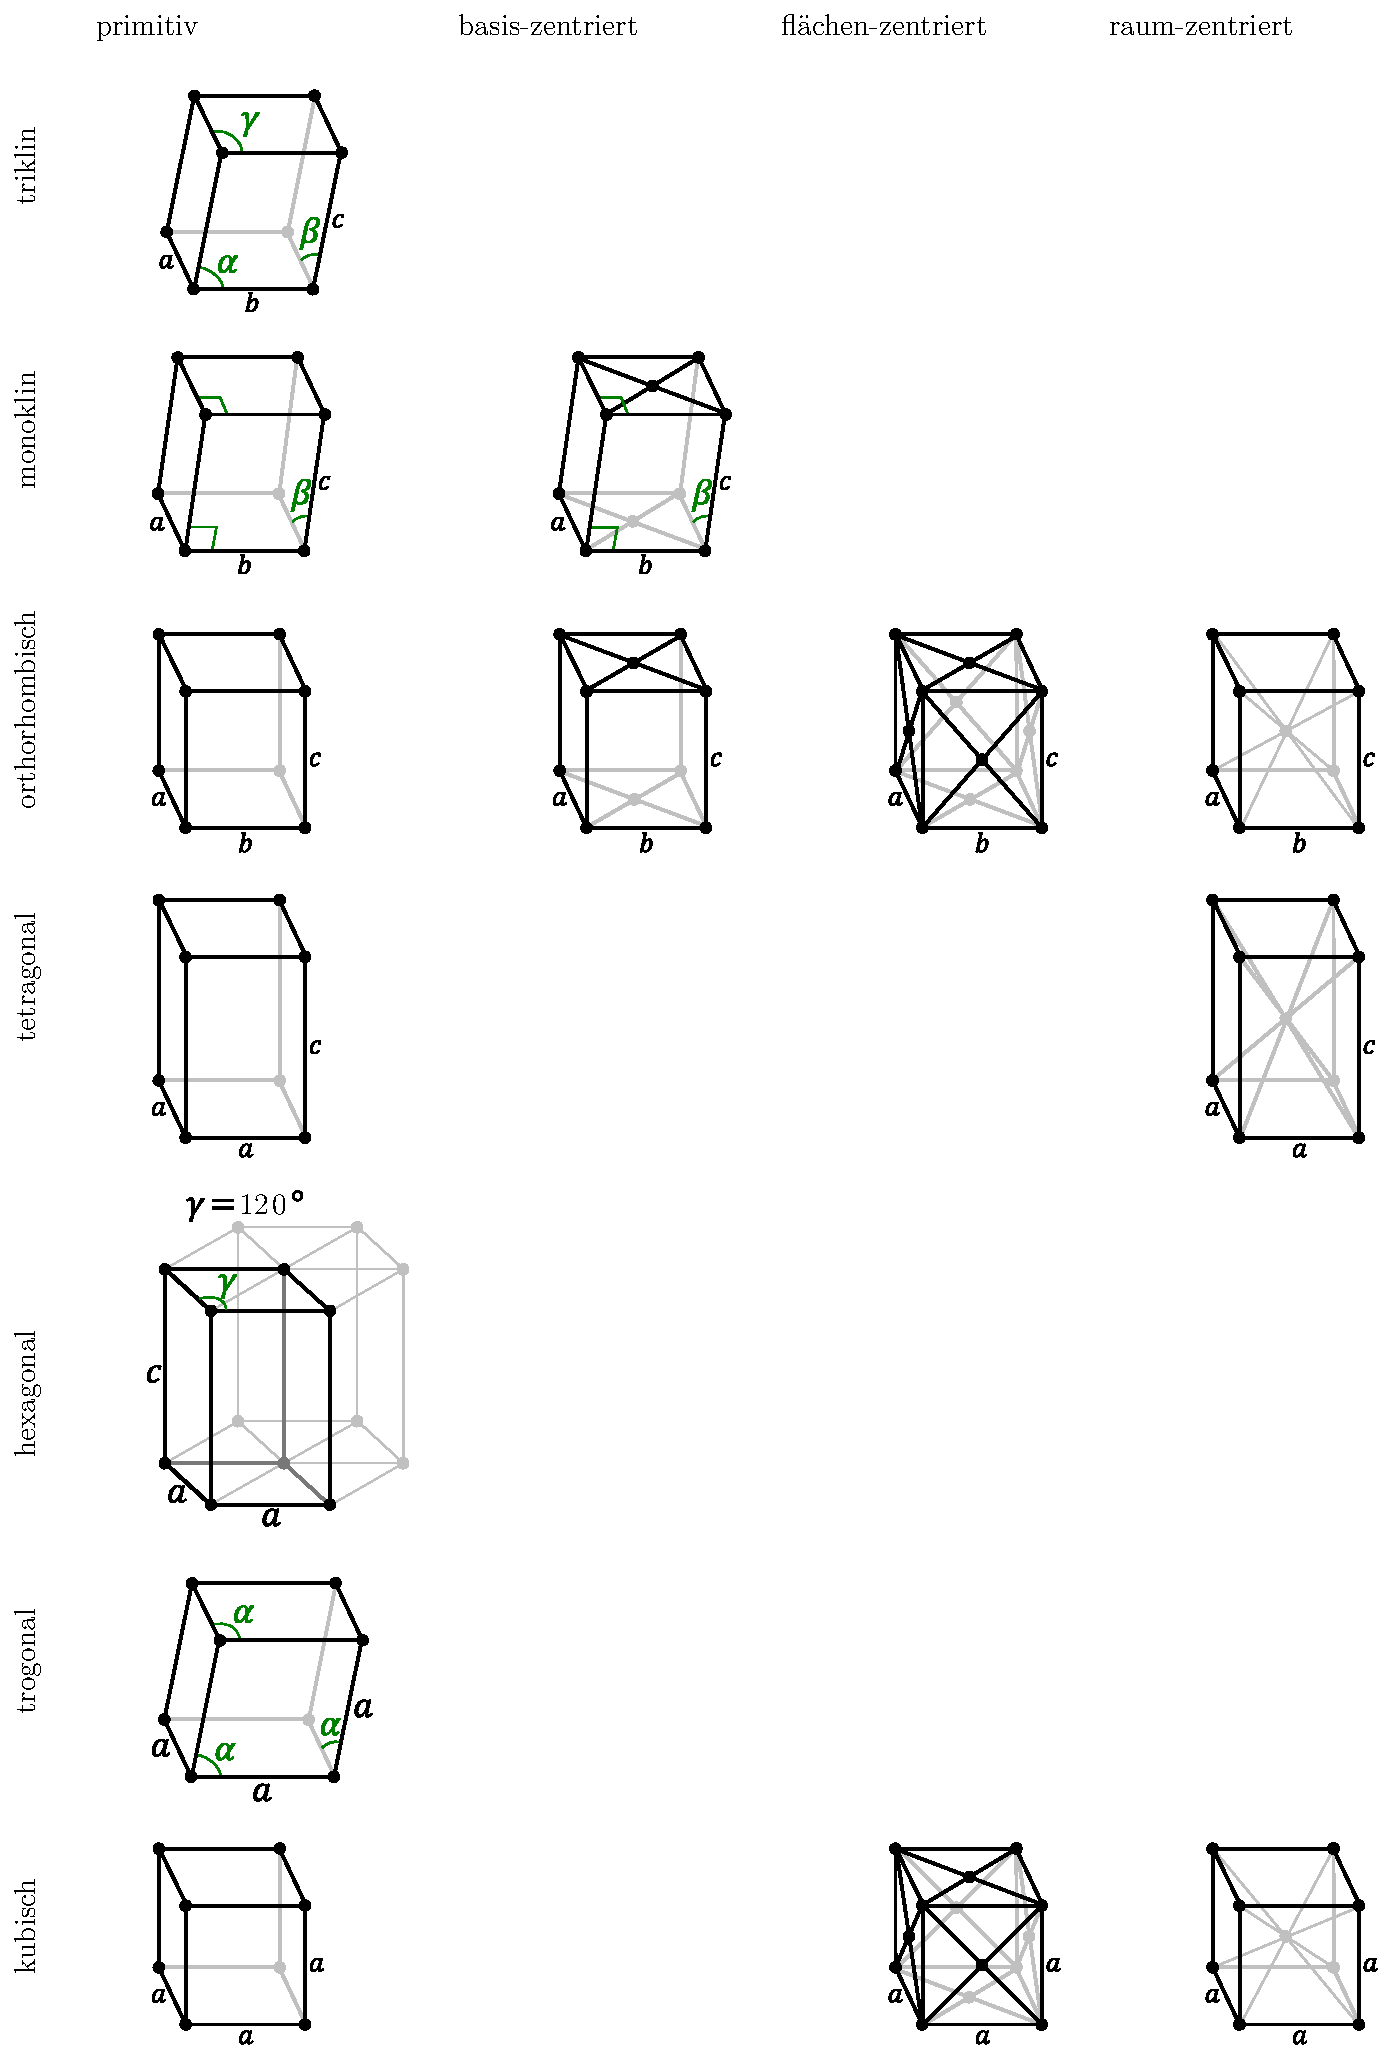
\includegraphics[height=\textheight]{\currfiledir kristall/bravais.pdf}
\inputtikz{\currfiledir bravais_ML}



\caption{Die 14 Bravais-Gitter. \label{fig:gitter_bravais14}  Gezeigt sind die konventionellen Einheitszellen, die die Symmetrie  des Gitters möglichst gut wiedergeben, aber im Falle der zentrierten Gitter nicht primitiv sind.
}
\end{figure}


\section{Die Basis}


Während das Gitter ein mathematisches Konstrukt ist, eine symmetrische Anordnung von mathematischen Punkten im dreidimensionalen Raum, kommt durch die \emph{Basis} die Natur ins Spiel. Die Basis beschreibt die Position der Atome relativ zum Gitterpunkt. Es kann dabei ein oder mehrere Atome in einer Basis sein. Die Position des Atoms $j$ relativ zum zugehörigen Gitterpunkt ist dann 
\begin{equation}
 \mathbf{r}_j = x_{1,j} \mathbf{a}_1 + x_{2,j} \mathbf{a}_2 + x_{3,j} \mathbf{a}_3  
\end{equation}
mit $0 \le x_{i,j} \le 1$. Die Lage der Atome in der Basis relativ zu 'ihrem' Gitterpunkt ist nicht eindeutig, da die Gitterpunkte ja mathematische Konstrukte und daher nicht messbar sind.


Die Symmetrie der Basis hat einen Einfluss auf die Symmetrie des Kristalls. Die sieben Kristallsysteme des mathematischen Gitters werden 32 kristallographische Punktgruppen, wenn also Translationssymmetrie unberücksichtigt bleibt. Diese unterscheiden sich dann in den anderen oben genannten Symmetrie-Operationen.
Wenn wieder die Translationssymmetrie mit berücksichtigen wird ergeben sich 230 kristallographische Raumgruppen.


\section{Beispiel: Honigwaben-Gitter}

Als Beispiel betrachten wir ein zweidimensionales Honigwaben-Gitter wie in nebenstehender Abbildung gezeigt. Dieses Gitter ist kein Bravais-Gitter, auch wenn es sehr symmetrisch aussieht. Zwei benachbarte Gitter-Punkte unterscheiden sich darin, wie das Gitter in ihrer Umgebung orientiert ist. Das  Honigwaben-Gitter ist ein dreizählig rotationssymmetrisches Gitter mit einer zwei-atomigen Basis. Mit dieser Wahl ist das Gitter translationsinvariant. Die Lage der Atome in der Basis relativ zu 'ihrem' Gitterpunkt ist nicht eindeutig. Die Skizze zeigt verschiedene Möglichkeiten.



\begin{marginfigure}
\inputtikz{\currfiledir honigwabe}

\caption{Honigwaben-Gitter}
\end{marginfigure}


\section{Die Wigner-Seitz-Zelle}

Die Wahl der primitiven Einheitszelle ist nicht eindeutig. Mit der Wigner-Seitz-Zelle gibt es eine Konstruktionsvorschrift, mit der man immer auf eine eindeutige primitive Einheitszelle kommt.



\begin{marginfigure}
\inputtikz{\currfiledir wsz-2d}

\caption{Konstruktion der Wigner-Seitz-Zelle in 2D.}
\end{marginfigure}

\begin{marginfigure}
\inputtikz{\currfiledir wsz-3d}

\caption{Die Wigner-Seitz-Zelle des raum-zentrierten kubischen Gitters.}
\end{marginfigure}

Man wähle einen Gitterpunkt und konstruiere Verbindungslinien zu allen benachbarten Punkten. Auf diese Linien errichte man Mittelsenkrechten (im zweidimensionalen) bzw. eine zur Linie senkrechte Ebene in der Mitte der Linie (im dreidimensionalen). Durch diese Mittelsenkrechten bzw. Mittelebenen wird eine Fläche bzw. ein Volumen eingeschlossen, das den Startpunkt beinhaltet. Dies ist die Wigner-Seitz-Zelle.

Diese Zelle ist primitiv, da sie nur einen Gitterpunkt beinhaltet. Sie hat außerdem die gleiche Symmetrie wie das Gitter selbst. Die Konstruktionsvorschrift ist unabhängig von der konkreten Wahl der Gittervektoren. Die Abbildungen zeigen als Beispiel die Konstruktion in einem schiefwinkligen zweidimensionalen Gitter sowie die Wigner-Seitz-Zelle des kubisch-raumzentrierten Gitters.


\section{Wichtige Kristallstrukturen}


\paragraph{\ch{NaCl}}
Kristallines \ch{NaCl} besteht aus einem flächen-zentrierten kubischen Gitter (engl: face-centered cubic, fcc). Schon weil es zwei verschiedene Atome sind muss es eine Basis mit mindestens zwei Atomen geben. Hier sind es genau zwei Atome,  beispielsweise mit \ch{Na+} im Ursprung und \ch{Cl-} im Zentrum der konventionellen Einheizstelle, also bei
\begin{equation}
 \mathbf{r}_{Cl} = \frac{1}{2} \left(\mathbf{a}_1 + \mathbf{a}_2 +  \mathbf{a}_3  \right)
\end{equation}
wenn die $\mathbf{a}_i$ so gewählt sind, dass sie die konventionelle Einheitszelle aufspannen, also kartesisch sind. Dies ist auch die Struktur von \ch{LiF}, \ch{MgO}, \ch{CaTe}.


\begin{marginfigure}
\inputtikz{\currfiledir nacl}

\caption{Kristallstruktur von \ch{NaCl}.}
\end{marginfigure}

\paragraph{\ch{CsCl}}
Dies ist ein primitives kubisches Gitter (engl. simple cubic, sc), ebenfalls mit einer zwei-atomigen Basis mit 
\begin{equation}
 \mathbf{r}_{Cl} = \frac{1}{2} \left(\mathbf{a}_1 + \mathbf{a}_2 +  \mathbf{a}_3  \right)
\end{equation}
Dies ist auch die Struktur von \ch{CsI}, \ch{TlBr}.

\begin{marginfigure}
\inputtikz{\currfiledir cscl}

\caption{Kristallstruktur von \ch{CsCl}.}
\end{marginfigure}

\paragraph{\ch{Fe}} Eisen bildet ein kubisch-raumzentriertes Gitter (engl. body-centered cubic, bcc) mit nur einem Atom in der Basis.

\paragraph{Diamant} Kohlenstoff-Atome in einem Diamant-Kristall bilden ein fcc-Gitter (face-centered cubic), aber ebenfalls mit einer zwei-atomigen Basis. Eine Basis kann also auch identische Atome beinhalten. Die Positionen sind der Ursprung sowie um ein Viertel der Raum-Diagonalen verschoben in der konventionellen Einheitszelle, als
\begin{align}
 \mathbf{r}_{C_1} = & 0 \\
 \mathbf{r}_{C_2} = & \frac{1}{4} \left(\mathbf{a}_1 + \mathbf{a}_2 +  \mathbf{a}_3  \right)
\end{align}
Die Atome sind untereinander in der tetraederförmigen Bindung der $sp^3$-Hybridisierung verbunden. Dies ist auch die Struktur von \ch{Si}, \ch{Ge}.

\begin{marginfigure}
\inputtikz{\currfiledir diamant}

\caption{Kristallstruktur von  Diamant (beide Atomsorten identisch) und Zinkblende (Atomsorten verschieden). Die Atome sind jeweils tetragonal gebunden, wie in dem Beispiel gezeigt.}
\end{marginfigure}

\paragraph{\ch{ZnS}} Zinkblende (\ch{ZnS}) hat die gleiche Struktur wie Diamant. Jede Atomsorte bildet für sich ein fcc-Gitter. Gegeneinander sind die Gitter um ein Viertel der Raum-Diagonalen verschoben. Dies ist auch die Struktur von \ch{CdTe}, \ch{GaAs}, \ch{InP}.


\section{Dichteste Kugelpackung}

Man kann die Atome in einem Kristallgitter durch harte Kugeln ersetzen und dabei den Kugeldurchmesser maximal wählen, also so, dass die Kugeln sich berühren. Welcher Volumenanteil des Kristalls wird nun durch Kugeln ausgefüllt? Die maximale Packungsdichte ist 
\begin{equation}
 \frac{\pi}{3 \sqrt{2}} \approx 74 \%
\end{equation}
Um diese Packungsdichte zu erreichen, liegen die Kugeln in der untersten Lage A in einem zweidimensionalen hexagonalen Gitter. Jede Kugel ist also von fünf Nachbarn umgeben. In der nächsten Lage B liegen die Kugeln in den Mulden, die sich zwischen den unteren Kugeln bilden.  Die Größe der Kugeln erzwingt, dass nur jeder zweite Mulde besetzt wird.
Dies ist wieder ein zweidimensionales hexagonales Gitter. Für die dritte Lage gibt es zwei Möglichkeiten: entweder man besetzt die Mulden, die den Positionen in Lage A entsprechen, oder man besetzt die Mulden, die weder von der Lage A noch von der Lage B eingenommen werden. Im ersten Fall spricht man von der ABAB-Stapelfolge, im zweiten von der ABCABC-Folge.

\begin{marginfigure}
\inputtikz{\currfiledir stacking}

\caption{ABC-Stapelfolge (oben) und ABA-Folge (unten).}
\end{marginfigure}


Welchen Bravais-Gittern entsprechen diese Folgen?  Die Folge ABCABC bildet ein flächen-zentriert kubisches Gitter (fcc).  Die Raumdiagonale der  Einheitszelle steht senkrecht auf den Ebenen A, B und C. Diese Packung wird daher auch 'cubic closed packing' (ccp) genannt. Die Folge ABAB nennt man  'hexagonal closed packing' (hcp), weil sie ein (dreidimensionales) hexagonales Bravais-Gitter mit einer zwei-atomigen Basis bildet (mit $c=a \sqrt{8/3}$, siehe Abb. \ref{fig:gitter_bravais14}). Eine Kugel ist dabei am Ursprung der konventionellen Einheitszelle, die zweite bei 
\begin{equation}
 \mathbf{r}_{S_2} =  \frac{2}{3}  \mathbf{a}_1 + \frac{1}{3}  \mathbf{a}_2 + \frac{1}{2}  \mathbf{a}_3  
\end{equation}
 wobei die $\mathbf{a}_i$ die konventionelle Einheitszelle aufspannen.

Die kubische dichteste Kugelpackung wird beispielsweise von \ch{Au} und \ch{Ag} realisiert, die hexagonal dichteste Kugelpackung von \ch{Cd} oder \ch{Mg}. Es finden sich auch komplexere Abfolgen der Positionen A, B und C. Metalle aus der Gruppe der seltenen Erden bilden beispielsweise ABACABAC.






\section{Bindungen in Festkörpern}



Wie bei den Molekülen  sind es auch in den Festkörpern die Elektronen der Atome, die die Bindung bewirken. Man kann die verschiedenen Bindungen also nach der Verteilung der Elektronen unterscheiden. Im Gegensatz zu Molekülen bilden sich Festkörper auch aus Atomen mit abgeschlossenen Schalen. Die schwache van-der-Waals-Kraft bildet beispielsweise Edelgaskristalle bei niedrigen Temperaturen. In Ionenkristallen wird ein Elektron transferiert und die Coulomb-Anziehung  bestimmt die Bindung. Die kovalente Bildung in Festkörpern ist analog zur der in Molekülen. Als Extremfall gibt es die metallische Bindung, bei der manche Elektronen über den ganzen Kristall gleichmäßig verteilt sind und  ein freies Elektronengas bilden. Ein Sonderfall ist die Wasserstoff-Brückenbindung, die aber in der Biologie eine große Rolle spielt. Im Folgenden werden wir die für uns neuen  Bindungen besprechen.

\begin{marginfigure}
\inputtikz{\currfiledir bindung}

\caption{Skizzenhafte Darstellung der Bindungstypen im Unterschied der Verteilung der Elektronen.}
\end{marginfigure}



\section{Van-der-Waals-Bindung}

Die Van-der-Waals-Bindung ist sehr schwach (meV pro Atom), aber immer vorhanden. Sie wird also nur dann sichtbare, wenn andere Bindungskräfte nicht zum Tragen kommen, beispielsweise in Kristallen von Edelgas-Atomen.

Die Verteilung der Elektronen um einen Atomkern ist kein starres Gebilde. Die Elektronendichte-Verteilung fluktuiert und in einem Augenblick kann es ein netto Dipolmoment $\mathbf{p}_1$ bei Atom $1$ geben. Dieses Dipolmoment ist verknüpft mit einem elektrischen Feld, dessen Amplitude $E_1 \propto p_1 / r^3$ ist.\sidenote{Die Richtungsabhängigkeit ignorieren wir hier.} Ein Atom $2$ in der Entfernung $r$ wird dann durch dieses Feld polarisiert und es bildet sich ein induziertes Dipolmoment $p_2 = \alpha E_1 \propto 1/r^3$. Das Wechselwirkungspotential $\phi(r)$ ist damit das Potential von $\mathbf{p}_2$ im Feld $\mathbf{E}_1$, 
\begin{equation}
 \phi(r) = - \mathbf{p}_2 \, \mathbf{E}_1 \propto - \frac{B}{r^6}
\end{equation}
wobei die Konstante $B$ positiv und für das jeweilige Element charakteristisch ist.

Bei kleine Atom--Atom--Abständen kommt die abstoßende Kraft aufgrund des Pauli-Verbots hinzu. Oft modelliert man sie als $A/r^{12}$. Insgesamt ergibt sich damit das \emph{Lenard-Jones-Potential}
\begin{equation}
\phi(r) = \frac{A}{r^{12}} - \frac{B}{r^{6}} = 4 \epsilon \left[ \frac{\sigma}{r^{12}} -  \frac{\sigma}{r^{6}} \right]
\end{equation}
wobei $\epsilon$ die Tiefe und $\sigma$ den Nulldurchgang des Potentials, sozusagen den Radius des Atomrumpfes, bestimmt. Der Gleichgewichtsabstand ist $r_0 = 2^{1/6} \sigma \approx 1.12 \sigma$.

In einem Kristall wirkt dieses Potential zwischen allen Paaren von Atomen, also ist die Bindungsenergie 
\begin{equation}
U_B = \frac{1}{2} \sum_{m,n}^N \phi_{n,m} = 
2 N \epsilon \sum_{m=1,   \neq n}^N 
\left[ 
\frac{\sigma}{r_{nm}^{12}} -  \frac{\sigma}{r_{nm}^{6}} 
\right]
\end{equation}
Der Faktor $1/2$ kommt daher, dass man in der ersten Summe alle Bindungs-Paare doppelt zählt. Die zweite Summe läuft nur noch über einen Summanden, da der Kristall translationsinvariant ist und es daher ausreicht, von einem Atom ausgehend alle Bindungen zu betrachten.

Dies lässt sich weiter vereinfachen, in dem man den Atom--Atom--Abstand $r_{nm}$ schreibt als $r_{nm} = \rho_{nm} \, a$  mit der Gitterkonstanten $a$ im kubischen flächenzentrierten (fcc) Gitter:
\begin{align}
U_B = & 
2 N \epsilon 
\left[ 
\frac{\sigma^{12}}{a^{12}}
\sum_{m=1,   \neq n}^N  \frac{1}{\rho_{nm}^{12}} 
-
\frac{\sigma^{6}}{a^{6}}
\sum_{m=1,   \neq n}^N  \frac{1}{\rho_{nm}^{6}} 
\right] \\
\approx & 
2 N \epsilon 
\left[ 
12.13 \; \frac{\sigma^{12}}{a^{12}}
-
14.45 \; \frac{\sigma^{6}}{a^{6}}
\right] 
\end{align}
Das Minimum der Bindungsenergie im Kristall findet sich nun bei $r_0 \approx 1.09 \sigma$, also etwas näher als im vd-Waals-'Molekül'. Dieser Wert wird auch experimentell für die schwereren Edelgasatome gefunden.

\section{Ionische Bindung}

Bei der Ionischen Bindung dominiert die Coulomb-Anziehung zwischen unterschiedlich geladenen Ionen. Die van-der-Waals-Wechselwirkung vernachlässigen wir also. Am Beispiel von \ch{NaCl} diskutieren wir die einzelnen Beiträge zur Bindungsenergie.

Zunächst müssen wir beide Atome ionisieren
\begin{align}
 \ch{Na} + 5.14\text{ eV} \rightarrow  & \ch{Na+} + \ch{e-} \\
  \ch{e-}  + \ch{Cl} \rightarrow  & \ch{Cl-} + 3.16\text{ eV}
\end{align}
Wir müssen also netto 1.53 eV aufwenden, um ein Ionenpaar herzustellen.

Dann bringen wir die beiden Ionen aus dem Unendlichen zusammen, bis zum experimentell gefundenen Bindungsabstand von $R_0 = 2.81$~\AA. Die Coulomb-Energie bei diesem Abstand beträgt -5.1~eV. Insgesamt gewinnen wir also durch Bildung eines \ch{NaCl}-'Moleküls' 3.57~eV. Dabei ist aber der abstoßende Teil des Bindungspotentials und die Wechselwirkung mit allen anderen Ionen des Kristalls noch nicht berücksichtigt.

Analog zur van-der-Waals-Wechselwirkung setzen wir also wieder als Potential zwischen einem Paar von Ionen an
\begin{equation}
 \phi(r_{nm}) = \pm \frac{e^2}{4 \pi \epsilon_0 \, r_{nm}} + \frac{B}{ r_{nm}^{12}}
\end{equation}
Das wechselnde Vorzeichen berücksichtigt die abwechselnd anziehende und abstoßende Wechselwirkung, je nach Ladung des Ions. Wir bilden wieder die Summe über alle Paare
\begin{equation}
U_B = N \sum_{m \neq n} \, \phi(r_{nm})  = N \sum_{m \neq n} \, \phi(\rho_{nm} \, a) 
\end{equation}
wobei $N$ nun die Anzahl der Ionen einer Sorte bezeichnet und so der Faktor 2 überflüssig wird. Wir haben wieder die Abstände durch die Gitterkonstante ausgedrückt. Nun machen wir die Annahme, dass die Abstoßende Wechselwirkung kurzreichweitig ist und nur $z$ Ionen im Abstand $a$ beitragen. Damit wird  
\begin{align}
U_B = & + z \frac{ B}{ a^{12}} - N \sum_{m \neq n} \, \pm \frac{e^2}{4 \pi \epsilon_0 \, \rho_{nm} \, a}  \\
= & + z \frac{ B}{ a^{12}} - N \frac{e^2}{4 \pi \epsilon_0 \,  \, a}  \, \alpha
\end{align}
mit der \emph{Madelung-Konstante} $\alpha$
\begin{equation}
 \alpha = \sum_{m \neq n} \, \frac{\pm}{\rho_{nm} }  
\end{equation}
Die Madelung-Konstante hängt nur von der Art des Gitters ab. Ihre Berechnung erfordert allerdings ein paar Tricks, da die Reihe insbesondere im Dreidimensionalen nicht gut konvergiert. 

\begin{marginfigure}

\begin{tabular}{ll}
kubisch flächen-z. & $\alpha \approx 1.747$ \\
kubisch raum-z. & $\alpha \approx 1.763$ \\
Diamant & $\alpha \approx 1.64$ \\
\end{tabular}
\caption{Die Madelung-Konstante $\alpha$ hängt nur schwach vom Gitter-Typ ab.}
\end{marginfigure}

Am Gleichgewichts-Abstand ist die Ableitung nach der Gitterkonstante Null, wodurch sich $B$ bestimmen lässt. Damit ergibt sich für die Bindungsenergie pro Ion einer Sorte
\begin{equation}
\frac{U_B}{N} = \frac{e^2 \, \alpha }{4 \pi \epsilon_0 \, R_0} \, \left( 1- \frac{1}{12} \right) = U_\text{Coulomb} \, \alpha \, \left( 1- \frac{1}{12} \right) 
\end{equation}
Für \ch{NaCl} ergibt sich so ein Wert von -8.25~eV, nah am experimentell gefundenen Wert von -8.15~eV.





\section{Wasserstoffbrückenbindung}

In einer Wasserstoffbrückenbindung bildet ein Wasserstoff-Atom nicht eine kovalente Bindung zu einem anderen Atom, sondern zu zwei Atomen. Dies ist natürlich keine gewöhnliche kovalente Bindung. Dazu fehlt dem Wasserstoff  Bindungselektron.

Die Wasserstoffbrückenbindung entsteht, wenn das H-Atom stark kovalent an einen Bindungspartner gebunden ist. Bei geht das Elektron des H-Atoms fast vollständig auf den Partner über und es verbleibt quasi ein Proton. Dies wirkt anziehend auf andere negativ geladene Bindungspartner. Aus räumlichen Gründen\sidenote{Das Proton ist viel kleiner als alle Atome mit Elektronen} kann jeweils nur ein weiterer Bindungspartner wechselwirken. Die Bindung ist daher auch oft asymmetrisch, also \ch{A}$-$\ch{H}$--$\ch{B}. Typische Bindungsenergien sind 0.2~eV, bei \ch{HF} kann aber auch 1.6~eV erreicht werden.

Diese Bindung spielt in der Biologie eine große Rolle. Proteine sind typischerweise durch viele Wasserstoffbrückenbindung verbunden. Jede einzelne Bindung ist schwach, nicht viel stärker als $k_B T$, und kann so einfach geöffnet werden, um eine Funktionalität zu erzeugen. Gleichzeitig sind alle Bindungen zusammen stark, ähnlich einem Klettverschluss.





%-------------------




\printbibliography[segment=\therefsegment,heading=subbibliography]
